\section{Approccio Multi-Livello}\label{sec:approccio-multi-livello}
In questa sezione verr\`a introdotto il concetto di contrazione a pi\`u livelli di grafi.
L'idea di base di un approccio multi-livello \`e quella di applicare ripetutamente operazioni di contrazione
da un grafo di partenza, ottenendo una sequenza di grafi contratti di dimensione via via minore.
Sebbene tale approccio sia stato generalmente utilizzato per ridurre la dimensione di un grafo al fine di
applicare efficientemente algoritmi di partizionamento~\cite{DBLP:journals/corr/abs-1012-0006},
non mancano esempi di applicazioni in contesti diversi, come quello della visualizzazione di grafi di grandi
dimensioni~\cite{4069239}.

In ogni caso, lo scopo di un approccio multi-livello \`e quello di costruire una gerarchia di grafi contratti
che rappresentino la struttura del grafo di partenza, comprimendo in nodi in meta-nodi in accordo a determinate
caratteristiche d'interesse.
Così come per la terminologia usata per le partizioni, i grafi risultanti dalle contrazioni sono spesso detti
grezzi (\textit{coarse}), mentre quelli risultanti dalle decontrazioni sono detti raffinati (\textit{fine}).
I grafi grezzi, ottenuti ricorsivamente a partire dai grafi pi\`u raffinati, sono quindi da considerarsi
come rappresentazioni pi\`u astratte di questi ultimi. \newline

\subsection{Partizionamento multi-livello di grafi}\label{subsec:partizionamento-multilivello-di-grafi}
Il \textbf{partizionamento multi-livello di grafi} (in inglese \textit{multilevel graph partitioning} o \textit{MGP})
\`e un approccio euristico per la risoluzione di problemi su grafi in cui si vuole dividere un grafo in un dato numero
di blocchi che abbiano approssimativamente la stessa dimensione, affinch\`e una certa funzione obiettivo sia
minimizzata.
Un esempio di tale problema dalla grande utilità pratica \`e quello in cui l'obiettivo del partizionamento consiste
nel minimizzare il numero di archi che connettono i blocchi.
Esso trova applicazione in importanti contesti legati all'informatica, ad esempio per la decomposizione di strutture
dati per la computazione parallela, e all'ingegneria, ad esempio per il partizionamento di circuiti integrati. \newline

L'approccio multi-livello, per la prima volta introdotto da Hendrickson e Leland nel
1995~\cite{Hendrickson1995}, si \`e rivelato essere quello di maggior successo per la risoluzione
di problemi di partizionamento di grafi di grandi dimensioni, in quanto permette di ottenere partizioni di alta
qualit\`a in tempi ragionevoli, nonostante il problema di partizionamento sia NP-completo per la maggior parte delle
funzioni obiettivo.
L'utilit\`a di questa tecnica si basa sull'intuizione per cui una buona partizione a un livello grezzo della
gerarchia rimarr\`a tale anche ad un livello pi\`u raffinato, e che, in questo modo, la ricerca di una
partizione ottimale pu\`o essere effettuata su grafi pi\`u piccoli e pi\`u semplici.
\newpage

\begin{figure}
    \centering
    

\tikzset{every picture/.style={line width=0.75pt}} %set default line width to 0.75pt

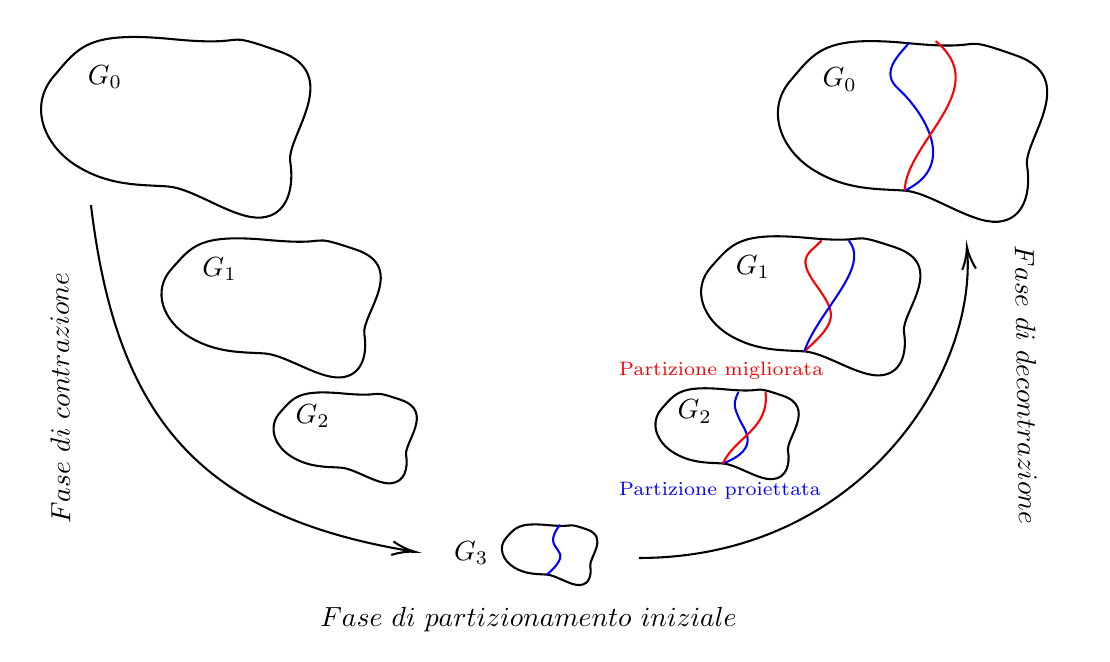
\begin{tikzpicture}[x=0.75pt,y=0.75pt,yscale=-1,xscale=1]
%uncomment if require: \path (0,301); %set diagram left start at 0, and has height of 301

%Shape: Polygon Curved [id:ds5681990127641572]
\draw   (13,23) .. controls (25,9) and (29,1) .. (70,5) .. controls (111,9) and (91,0) .. (122,11) .. controls (153,22) and (125.09,51.89) .. (127,64) .. controls (128.91,76.11) and (126,90) .. (113,91) .. controls (100,92) and (80.66,76.9) .. (68,76) .. controls (55.34,75.1) and (40,76) .. (24,66) .. controls (8,56) and (1,37) .. (13,23) -- cycle ;
%Shape: Polygon Curved [id:ds5791880784550985]
\draw   (69.88,115.65) .. controls (79.65,104.87) and (82.9,98.71) .. (116.29,101.79) .. controls (149.67,104.87) and (133.38,97.94) .. (158.63,106.41) .. controls (183.87,114.88) and (161.14,137.9) .. (162.7,147.22) .. controls (164.25,156.55) and (161.88,167.24) .. (151.3,168.01) .. controls (140.71,168.78) and (124.96,157.16) .. (114.66,156.46) .. controls (104.35,155.77) and (91.86,156.46) .. (78.83,148.76) .. controls (65.81,141.06) and (60.11,126.43) .. (69.88,115.65) -- cycle ;
%Shape: Polygon Curved [id:ds8471099289598505]
\draw   (122.17,184.81) .. controls (128.56,177.76) and (130.68,173.74) .. (152.5,175.75) .. controls (174.32,177.76) and (163.67,173.23) .. (180.17,178.77) .. controls (196.67,184.3) and (181.81,199.34) .. (182.83,205.44) .. controls (183.85,211.53) and (182.3,218.52) .. (175.38,219.02) .. controls (168.46,219.53) and (158.17,211.93) .. (151.44,211.48) .. controls (144.7,211.02) and (136.54,211.48) .. (128.02,206.44) .. controls (119.51,201.41) and (115.79,191.85) .. (122.17,184.81) -- cycle ;
%Shape: Polygon Curved [id:ds042557391147138635]
\draw   (231.1,245.21) .. controls (235.36,240.51) and (236.78,237.83) .. (251.33,239.17) .. controls (265.87,240.51) and (258.78,237.49) .. (269.78,241.19) .. controls (280.78,244.88) and (270.87,254.91) .. (271.55,258.97) .. controls (272.23,263.04) and (271.2,267.7) .. (266.58,268.03) .. controls (261.97,268.37) and (255.11,263.3) .. (250.62,263) .. controls (246.13,262.69) and (240.68,263) .. (235,259.64) .. controls (229.32,256.29) and (226.84,249.91) .. (231.1,245.21) -- cycle ;
%Shape: Polygon Curved [id:ds19971791116540039]
\draw   (368,25) .. controls (380,11) and (384,3) .. (425,7) .. controls (466,11) and (446,2) .. (477,13) .. controls (508,24) and (480.09,53.89) .. (482,66) .. controls (483.91,78.11) and (481,92) .. (468,93) .. controls (455,94) and (435.66,78.9) .. (423,78) .. controls (410.34,77.1) and (395,78) .. (379,68) .. controls (363,58) and (356,39) .. (368,25) -- cycle ;
%Shape: Polygon Curved [id:ds6697871941207159]
\draw   (329.88,114.65) .. controls (339.65,103.87) and (342.9,97.71) .. (376.29,100.79) .. controls (409.67,103.87) and (393.38,96.94) .. (418.63,105.41) .. controls (443.87,113.88) and (421.14,136.9) .. (422.7,146.22) .. controls (424.25,155.55) and (421.88,166.24) .. (411.3,167.01) .. controls (400.71,167.78) and (384.96,156.16) .. (374.66,155.46) .. controls (364.35,154.77) and (351.86,155.46) .. (338.83,147.76) .. controls (325.81,140.06) and (320.11,125.43) .. (329.88,114.65) -- cycle ;
%Shape: Polygon Curved [id:ds6317966254041107]
\draw   (306.17,182.81) .. controls (312.56,175.76) and (314.68,171.74) .. (336.5,173.75) .. controls (358.32,175.76) and (347.67,171.23) .. (364.17,176.77) .. controls (380.67,182.3) and (365.81,197.34) .. (366.83,203.44) .. controls (367.85,209.53) and (366.3,216.52) .. (359.38,217.02) .. controls (352.46,217.53) and (342.17,209.93) .. (335.44,209.48) .. controls (328.7,209.02) and (320.54,209.48) .. (312.02,204.44) .. controls (303.51,199.41) and (299.79,189.85) .. (306.17,182.81) -- cycle ;
%Curve Lines [id:da4556621139317687]
\draw [color={rgb, 255:red, 0; green, 0; blue, 255 }  ,draw opacity=1 ]   (250.62,263) .. controls (267,249) and (246,253) .. (257,239) ;
%Curve Lines [id:da3153745771749539]
\draw [color={rgb, 255:red, 0; green, 0; blue, 255 }  ,draw opacity=1 ]   (335.44,209.48) .. controls (355,202) and (345.05,192.39) .. (343.35,188.03) .. controls (341.65,183.68) and (339.62,181.49) .. (343,175) ;
%Curve Lines [id:da24590148322887484]
\draw [color={rgb, 255:red, 255; green, 0; blue, 0 }  ,draw opacity=1 ]   (335.44,209.48) .. controls (341.44,196.48) and (358,193) .. (356,175) ;
%Curve Lines [id:da8069367964557173]
\draw [color={rgb, 255:red, 255; green, 0; blue, 0 }  ,draw opacity=1 ]   (374.66,155.46) .. controls (391.66,140.46) and (390,137) .. (380,123) .. controls (370,109) and (378,108) .. (383,102) ;
%Curve Lines [id:da030698152549456736]
\draw [color={rgb, 255:red, 0; green, 0; blue, 255 }  ,draw opacity=1 ]   (374.66,155.46) .. controls (381.66,135.46) and (407,115) .. (396,102) ;
%Curve Lines [id:da9188529841976845]
\draw [color={rgb, 255:red, 0; green, 0; blue, 255 }  ,draw opacity=1 ]   (423,78) .. controls (451,65) and (429,37) .. (420,29) .. controls (411,21) and (420,13) .. (425,7) ;
%Curve Lines [id:da500049878186364]
\draw [color={rgb, 255:red, 255; green, 0; blue, 0 }  ,draw opacity=1 ]   (423,78) .. controls (424,54) and (466,29) .. (438,6) ;
%Curve Lines [id:da5337953441131338]
\draw    (31,85) .. controls (42.94,184.5) and (80.62,234.5) .. (185.42,251.74) ;
\draw [shift={(187,252)}, rotate = 189.11] [color={rgb, 255:red, 0; green, 0; blue, 0 }  ][line width=0.75]    (10.93,-3.29) .. controls (6.95,-1.4) and (3.31,-0.3) .. (0,0) .. controls (3.31,0.3) and (6.95,1.4) .. (10.93,3.29)   ;
%Curve Lines [id:da17376352225172775]
\draw    (295,255) .. controls (400.93,255) and (457.86,166.79) .. (453.16,106.81) ;
\draw [shift={(453,105)}, rotate = 84.29] [color={rgb, 255:red, 0; green, 0; blue, 0 }  ][line width=0.75]    (10.93,-3.29) .. controls (6.95,-1.4) and (3.31,-0.3) .. (0,0) .. controls (3.31,0.3) and (6.95,1.4) .. (10.93,3.29)   ;

% Text Node
\draw (28,16.4) node [anchor=north west][inner sep=0.75pt]    {$G_{0}$};
% Text Node
\draw (83.23,108.82) node [anchor=north west][inner sep=0.75pt]    {$G_{1}$};
% Text Node
\draw (128.13,179.36) node [anchor=north west][inner sep=0.75pt]    {$G_{2}$};
% Text Node
\draw (204.41,245.38) node [anchor=north west][inner sep=0.75pt]    {$G_{3}$};
% Text Node
\draw (382,17.4) node [anchor=north west][inner sep=0.75pt]    {$G_{0}$};
% Text Node
\draw (340.23,107.82) node [anchor=north west][inner sep=0.75pt]    {$G_{1}$};
% Text Node
\draw (312.13,177.36) node [anchor=north west][inner sep=0.75pt]    {$G_{2}$};
% Text Node
\draw (10.34,240.07) node [anchor=north west][inner sep=0.75pt]  [rotate=-269.56]  {$Fase\ di\ contrazione$};
% Text Node
\draw (486.92,102.91) node [anchor=north west][inner sep=0.75pt]  [rotate=-89.15]  {$Fase\ di\ decontrazione$};
% Text Node
\draw (140,277.4) node [anchor=north west][inner sep=0.75pt]    {$Fase\ di\ partizionamento\ iniziale$};
% Text Node
\draw (284,217) node [anchor=north west][inner sep=0.75pt]   [align=left] {{\scriptsize \textcolor[rgb]{0,0,1}{Partizione proiettata}}};
% Text Node
\draw (284,159) node [anchor=north west][inner sep=0.75pt]  [font=\normalsize] [align=left] {{\scriptsize \textcolor[rgb]{1,0,0}{Partizione migliorata}}};


\end{tikzpicture}

    \caption{Schema grafico del partizionamento multilivello}
    \label{fig:multi-level-graph-partitioning}
\end{figure}

L'approccio multi-livello per la partizione di grafi si articola in tre fasi principali:
\begin{enumerate}
    \item \textbf{Fase di contrazione} (\textit{contraction/coarsening phase}):
    si crea una gerarchia di grafi riducendo iterativamente la dimensione del grafo iniziale.
    Questo viene fatto comunemente individuando e contraendo coppie di nodi adiacenti, ovvero individuando un
    sottoinsieme degli archi del grafo da contrarre, $M \subseteq E $ detti \textit{match}.
    Si noti che la scelta di contrarre coppie di nodi adiacenti porta a grafi grossolani i cui nodi rappresentano
    sottografi del grafo iniziale densamente connessi.
    In base allo specifico problema, una determinata funzione di \textit{rating} classifica gli archi individuando
    quale sottoinsieme degli archi $E$ debba essere assegnato ad $M$ affinch\`e la somma dei \textit{rating} degli in
    $M$ sia globalmente massimizzata.
    Si consideri che un nodo gi\`a contratto non pu\`o essere pi\`u coinvolto in un ulteriore \textit{matching}
    allo stesso livello della gerarchia.
    \item \textbf{Fase di partizionamento iniziale} (\textit{initial partitioning phase}): quando a seguito delle
    contrazioni il grafo risulta essere di ordine abbastanza piccolo, in relazione ad un qualche threshold,
    esso pu\`o essere partizionato direttamente con algoritmi costosi, fornendo una partizione iniziale sul grafo
    pi\`u grossolano della gerarchia.
    \item \textbf{Fase di decontrazione} (\textit{refinement/uncoarsening phase}), i matching vengono iterativamente
    decontratti, e i relativi nodi vengono associati a blocchi della partizione del grafo pi\`u grossolano,
    proiettandola sul grafo pi\`u raffinato.
    Per fare in modo che la partizione al livello pi\`u grossolano tenga conto delle sotto-strutture ai livelli
    pi\`u raffinati, un algoritmo di miglioramento locale (\textit{local improvement}) ricolloca i nodi tra i
    blocchi per migliorare la dimensione del taglio o l'equilibrio delle dimensioni tra i blocchi.
\end{enumerate}